This section describes the purpose, use and intended user audience for the Smart Cart. The Smart Cart is an autonomous system that will help carry and power tools. Users of the Smart Cart will be able to use it to hold demonstrations outdoors.

\subsection{Purpose and Use}
The Smart Cart will provide assistance by being an autonomous carrier. The cart needs to be able to do the following things:
\begin{itemize}
	\item Follow a ''master'' to the designated destination
	\item Avoid collision with obstacles such as walls and other people
	\item Include an integrated power supply
	\item Holonomic mobility
\end{itemize}


\subsection{Intended Audience}
This is where you describe the intended audience(s) of your product. If this product were to be made available publicly or commercially, who would purchase or use it? Is the product designed for a particular customer, or an overall class of customers? Is it intended for general use, or is it a specific component of a more complex system?

\begin{figure}[h!]
	\centering
   	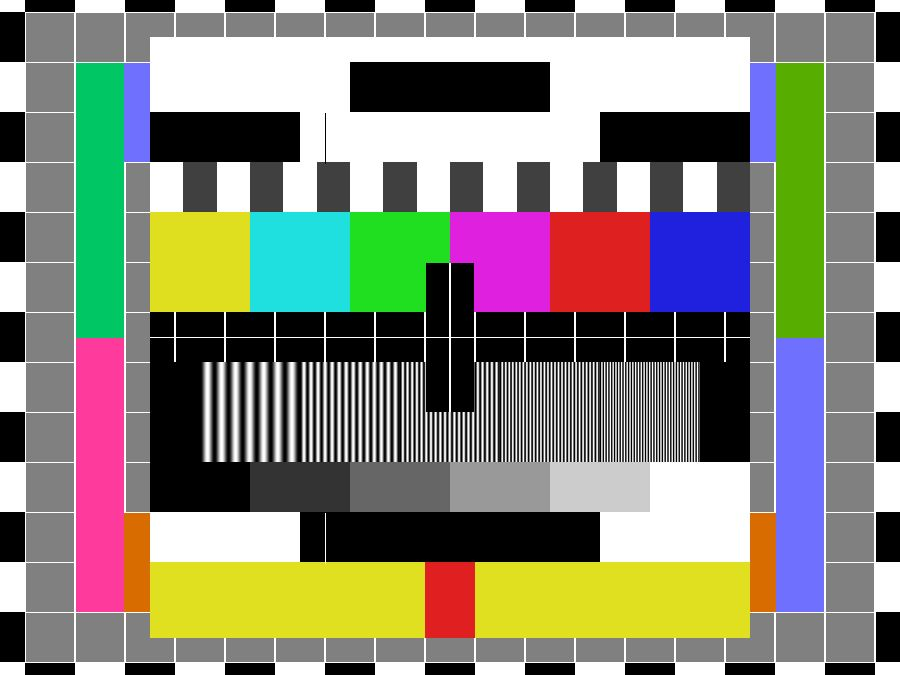
\includegraphics[width=0.60\textwidth]{images/test_image}
    \caption{X conceptual drawing}
\end{figure}
